% NoiseMap: schematický diagram architektúry (zdroj pre diagram.pdf)
% Preklad: pdflatex diagram.tex  (alebo xelatex diagram.tex)  ->  diagram.pdf
\documentclass[tikz,border=4pt]{standalone}

\usepackage{iftex}
\ifXeTeX
  \usepackage{fontspec}
  \setsansfont{Latin Modern Sans}
\else
  \usepackage[T1]{fontenc}
  \usepackage[utf8]{inputenc}
  \usepackage{lmodern} % vektorové písmo s diakritikou
\fi
\renewcommand{\familydefault}{\sfdefault} % rovnaké bezpätkové písmo ako v beameri

\usetikzlibrary{positioning,shapes.geometric,arrows.meta,fit,backgrounds,calc}

\definecolor{nmmodra}{RGB}{38,70,120}
\definecolor{nmsvetla}{RGB}{226,233,245}
\definecolor{nmzelena}{RGB}{220,238,224}
\definecolor{nmzelenat}{RGB}{40,100,60}
\definecolor{nmoranz}{RGB}{252,236,214}
\definecolor{nmoranzt}{RGB}{150,80,10}

\begin{document}
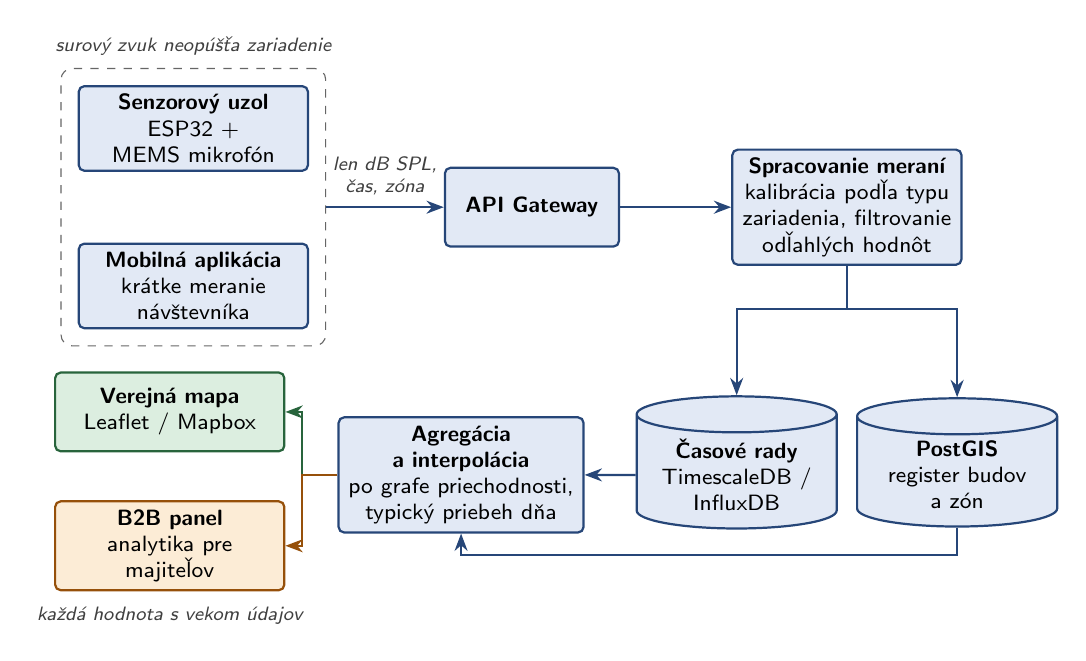
\begin{tikzpicture}[
  font=\footnotesize,
  >={Stealth[length=2.2mm]},
  box/.style={draw=nmmodra, fill=nmsvetla, rounded corners=2pt, thick,
              align=center, minimum height=10mm, text width=27mm, inner sep=3pt},
  db/.style={cylinder, shape border rotate=90, aspect=0.18, draw=nmmodra,
             fill=nmsvetla, thick, align=center, text width=24mm,
             minimum height=12mm, inner sep=2pt},
  b2c/.style={box, draw=nmzelenat, fill=nmzelena},
  b2b/.style={box, draw=nmoranzt, fill=nmoranz},
  tok/.style={->, thick, draw=nmmodra},
  popis/.style={font=\scriptsize\itshape, text=black!75, align=center}
]

% ---------- 1. riadok: zber a príjem meraní ----------
\node[box] (uzol)  at (0, 1.0)  {\textbf{Senzorový uzol}\\ESP32 + MEMS mikrofón};
\node[box] (mobil) at (0,-1.0)  {\textbf{Mobilná aplikácia}\\krátke meranie návštevníka};

\node[box, text width=20mm] (api) at (4.3,0) {\textbf{API Gateway}};
\node[box] (spr) at (8.3,0) {\textbf{Spracovanie meraní}\\kalibrácia podľa typu zariadenia, filtrovanie odľahlých hodnôt};

% hranica súkromia okolo zdrojov
\begin{scope}[on background layer]
  \node[draw=black!60, dashed, rounded corners=4pt, inner sep=6pt,
        fit=(uzol)(mobil)] (zariadenie) {};
\end{scope}
\node[popis, above=1pt of zariadenie.north] {surový zvuk neopúšťa zariadenie};

% šípka do API Gateway
\draw[tok] (zariadenie.east) -- (api.west);
\node[popis, above=1pt] at ($(zariadenie.east)!0.5!(api.west)$) {len dB SPL,\\čas, zóna};

\draw[tok] (api) -- (spr);

% ---------- 2. riadok: uloženie, analýza, výstupy ----------
\node[db] (ts)  at (6.9,-3.4) {\textbf{Časové rady}\\TimescaleDB /\\InfluxDB};
\node[db] (gis) at (9.7,-3.4) {\textbf{PostGIS}\\register budov\\a zón};

\node[box, text width=29mm] (agr) at (3.4,-3.4) {\textbf{Agregácia\\a interpolácia}\\po grafe priechodnosti,\\typický priebeh dňa};

\node[b2c] (mapa) at (-0.3,-2.6) {\textbf{Verejná mapa}\\Leaflet / Mapbox};
\node[b2b] (b2b)  at (-0.3,-4.3) {\textbf{B2B panel}\\analytika pre majiteľov};

\draw[tok] (spr.south) -- ++(0,-0.55) -| (ts.north);
\draw[tok] (spr.south) -- ++(0,-0.55) -| (gis.north);
\draw[tok] (ts.west) -- (agr.east);
\draw[tok] (gis.south) -- ++(0,-0.35) -| (agr.south);

\draw[tok, draw=nmzelenat] (agr.west) -- ++(-0.45,0) |- (mapa.east);
\draw[tok, draw=nmoranzt]  (agr.west) -- ++(-0.45,0) |- (b2b.east);

\node[popis, below=2pt of b2b.south] {každá hodnota s vekom údajov};

\end{tikzpicture}
\end{document}
